\subsection{Caso d'uso UC10: Salvataggio infografica}
\begin{figure}[h] 
	\centering 
	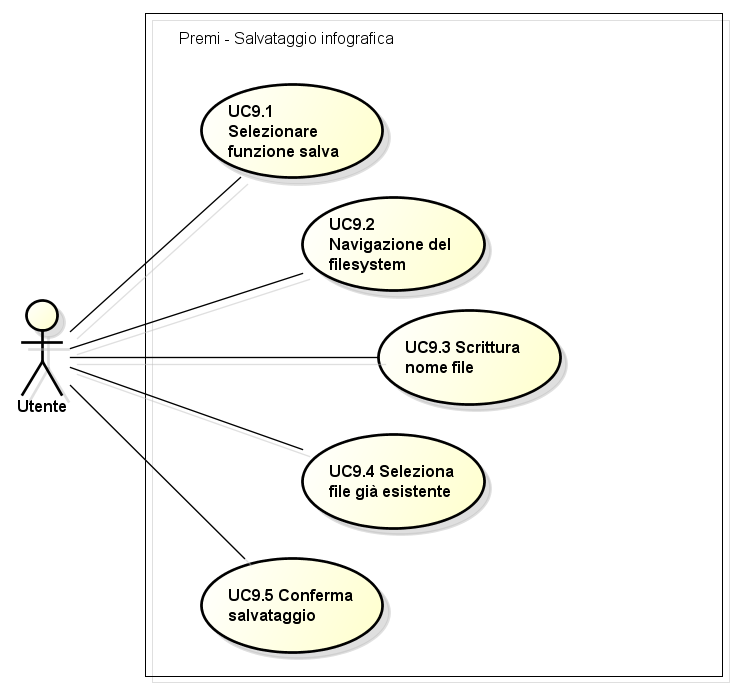
\includegraphics[scale=0.45] {img/UC10.png} 
	\caption{UC10 - Salvataggio infografica} 
\end{figure}

\begin{itemize}
	\item \textbf{Attori:} Utente;
	\item \textbf{Scopo e descrizione:} L'utente ha creato un'\gls{infografica} e vuole salvarla in una specifica cartella;
	\item \textbf{Precondizione:} Il sistema è in attesa che l'utente selezioni la funzione salva;
	\item \textbf{Flusso degli eventi:}
	\begin{enumerate}
		\item L'utente seleziona la funzione salva [UC10.1];
		\item L'utente seleziona la cartella nella quale salvare l'\gls{infografica} [UC10.2];
		\item L'utente scrive il nome del file [UC10.3];
		\item L'utente può selezionare un file già esistente da sovrascrivere [UC10.4];
		\item L'utente conferma il salvataggio [UC10.5].
	\end{enumerate}
	\item \textbf{Postcondizione:} Il sistema salvato l'\gls{infografica} nella cartella selezionata con il nome indicato.
\end{itemize}

\subsection{Caso d'uso UC10.1: Selezionare funzione salva}
\begin{itemize}
	\item \textbf{Attori:} Utente;
	\item \textbf{Scopo e descrizione:} L'utente seleziona dall'apposito menù la funzione di salvataggio per salvare l'\gls{infografica};
	\item \textbf{Precondizione:} Il sistema è in attesa che l'utente selezioni la funzione salva;
	\item \textbf{Postcondizione:} Il sistema apre la finestra di dialogo per il salvataggio.
\end{itemize}

\subsection{Caso d'uso UC10.2: Navigazione nel filesystem}
\begin{itemize}
	\item \textbf{Attori:} Utente;
	\item \textbf{Scopo e descrizione:} L'utente naviga il \gls{filesystem} per selezionare posizione di salvataggio dell'\gls{infografica};
	\item \textbf{Precondizione:} Il sistema è in attesa che l'utente selezioni una cartella;
	\item \textbf{Postcondizione:} Il sistema aggiorna il percorso con quello scelto dall'utente.
\end{itemize}

\subsection{Caso d'uso UC10.3: Scrittura nome file}
\begin{itemize}
	\item \textbf{Attori:} Utente;
	\item \textbf{Scopo e descrizione:} L'utente deve inserire un nome valido con il quale salvare l'\gls{infografica};
	\item \textbf{Precondizione:} Il sistema permette all'utente di selezionare il nome dell'\gls{infografica} da salvare;
	\item \textbf{Postcondizione:} È stato inserito un nome valido per l'\gls{infografica} che l'utente desidera salvare.
\end{itemize}

\subsection{Caso d'uso UC10.4: Seleziona file già esistente}
\begin{itemize}
	\item \textbf{Attori:} Utente;
	\item \textbf{Scopo e descrizione:} L'utente può selezionare un'\gls{infografica} già esistente da sovrascrivere con il salvataggio;
	\item \textbf{Precondizione:} Il sistema contiene già un'\gls{infografica} con il nome che l'utente desidera utilizzare;
	\item \textbf{Postcondizione:} L'\gls{infografica} già esistente è stata selezionata dall'utente.
\end{itemize}

\subsection{Caso d'uso UC10.5: Conferma salvataggio}
\begin{itemize}
	\item \textbf{Attori:} Utente;
	\item \textbf{Scopo e descrizione:} L'utente conferma il salvataggio dell'\gls{infografica};
	\item \textbf{Precondizione:} Il sistema ha ricevuto la richiesta di salvataggio dell'\gls{infografica};
	\item \textbf{Postcondizione:} Il sistema ha salvato l'\gls{infografica} selezionata dall'utente.
\end{itemize}